\documentclass[12pt,lot,lof]{puthesis}
\usepackage{amsfonts}
\usepackage{amssymb}
\usepackage{amsmath}
\usepackage{amsthm}
\usepackage{caption}
\usepackage{latexsym}
%\usepackage{graphicx}
%\usepackage{biblatex}


\usepackage{paralist}
\usepackage{tabularx}
\usepackage{multicol}
\usepackage{multirow}
\usepackage{booktabs}
\usepackage{color}

\usepackage{makecell}
\usepackage{pgf-pie}
\usepackage{listings}
\usepackage{pifont}
\usetikzlibrary{shadows}
\usepackage[hidelinks]{hyperref}
\usepackage[acronym, section]{glossaries}
\usepackage{natbib}

\setcitestyle{numbers}

\usepackage{citeref}


%\usepackage{setspace}
%\usepackage[round, longnamesfirst]{natbib} % for nice bibliography

%\input{./template/newcommands}

\newcommand{\puteqnum}{   
    \refstepcounter{equation}\textup{(\theequation)}}

% ================================================
% Table settings
\newcommand{\mysettingTableFont}{10}
\newcommand{\mysettingTableFontBaseline}{12}

\newcommand{\myTableStart}{\toprule}
\newcommand{\myTableHeaderSep}{\midrule\midrule}
\newcommand{\myTableSectionSep}{\midrule}
\newcommand{\myTableEnding}{\bottomrule}

\newcolumntype{Y}{>{\centering\arraybackslash}X}
% ================================================

\newcommand{\mylstinputlistingIDA}[2]{
    \setstretch{1.0}
    \lstset{language=IDA, style=lstPythonStyle}
    \lstinputlisting[language=IDA, caption={#2},captionpos=b]{#1}
    \setstretch{1.5}
}
\newcommand{\mylstinputlistingPython}[2]{
    \setstretch{1.0}
    \lstset{language=Python, style=lstPythonStyle}
    \lstinputlisting[language=Python, caption={#2},captionpos=b,label=#1]{#1}
    \setstretch{1.5}
}


\definecolor{codegreen}{rgb}{0,0.6,0}
\definecolor{codegray}{rgb}{0.5,0.5,0.5}
\definecolor{codepurple}{rgb}{0.58,0,0.82}
\definecolor{backcolour}{rgb}{0.95,0.95,0.92}

\lstdefinelanguage{IDA}{
    language=Python,
    morecomment=[l]{//}
}
\lstdefinestyle{lstPythonStyle}{
    commentstyle=\color{codegreen},
    keywordstyle=\color{magenta},
    numberstyle=\tiny\color{codegray},
    stringstyle=\color{codepurple},
    basicstyle=\ttfamily\footnotesize,
    breakatwhitespace=false,
    breaklines=true,
    captionpos=b,
    keepspaces=true,
    numbers=left,
    numbersep=5pt,
    showspaces=false,
    showstringspaces=false,
    showtabs=false,
    tabsize=2
}

% \title{}
\title{Model Explanation Methods for Decision Support in Demand Forecasting}
\submitted{2025}  %graduation date
\author{Mátyás Kuti-Kreszács}
\advisor{Prof. Dr. Dioșan Laura} %
\keywords{demand forecasting, explainable AI, decision support, machine learning, time series forecasting}
 \dedication{Dedicated to ..}


\abstract{
    
TODO: include
}

\acknowledgements{
%    \input{tex/acknow}
    
TODO: include
}

%\input{
%    chapters/glossary.tex
%}



\begin{document}

    \sloppy

% \setstretch{1.5}

% <<<<<<<<<<<<<<<<<<
% Publications
% \chapter*{List of publications}
% \input{tex/publications}
% \clearpage
% >>>>>>>>>>>>>>>>>>


% <<<<<<<<<<<<<<<<<<
% \printglossary
    \glsaddall
    \printglossary[type=\acronymtype, title={Acronyms}, nonumberlist]
% \printglossary[type=main, title={Glossary}]
    \printglossary[type=main, title={Glossary}, nonumberlist]
% >>>>>>>>>>>>>>>>>>

%    \input{tex/document}
    
\chapter{Introduction}\label{ch:introduction}
%
%\chapter{Introduction}
%\label{ch:introduction}

%test
Product demand forecasting is a common business problem in many industries.
But especially in production planning, manufacturing, logistics, inventory management, retail, and marketing.

Test citation~\cite{ketkar2017introduction}.

\section[Objectives]{Objectives}

% state the aim; the main objective of the research
% Options:
% - Have an "AIm statement", eg. "The aim of this research is to..."
% - Have a "Research question", eg. "The research questions,"  list of questions
% - Hipothesis, eg. "The hypothesis of this research is that..."



\section[Contributions]{Contributions}


\section[Publications]{List of Publications}


% list of publications that are part of the thesis


\section[Thesis Structure]{Thesis Structure}
\tectcolor{red}{TODO: describe the structure in the end}

% describe the structure of the thesis


\section[Introduction]{Introduction}\label{sec:introduction}
%\section{Motivation}
%\section{Objectives}
%\section{Contributions}

%\chapter{Introduction}
%\label{ch:introduction}

%test
Product demand forecasting is a common business problem in many industries.
But especially in production planning, manufacturing, logistics, inventory management, retail, and marketing.

%Test citation~\cite{ketkar2017introduction}.

\section[Objectives]{Objectives}


% state the aim; the main objective of the research
% Options:
% - Have an "AIm statement", eg. "The aim of this research is to..."
% - Have a "Research question", eg. "The research questions,"  list of questions
% - Hipothesis, eg. "The hypothesis of this research is that..."

The motivation of the thesis comes from the need to improve the explainability of machine learning forecasting models in order to raise trust in the system and deliver actionable insights for decision support.



\section[Contributions]{Contributions}

% list the contributions of the thesis
\begin{itemize}
    \item Contribution 1: Challenges in explainable AI for demand forecasting
    \item Contribution 2: Hierarchical feature importance in demand forecasting
    \item Contribution 3: Delivering actionable insights for decision support
\end{itemize}




% list of publications that are part of the thesis


\section[Thesis Structure]{Thesis Structure}
\textcolor{red}{TODO: describe the structure in the end}

% describe the structure of the thesis




\section[Publications]{List of Publications}\label{sec:publications}
% Own articles




\begin{itemize}
    \item \textbf{Category B Conference} – 4p \textcolor{red}{Workshop Proceedings (C) – 2p} % Consider clarifying this category
    \begin{itemize}
        \item M. Kuti-Kreszács, \emph{Optimising Hierarchical Demand Forecasting with Explainable AI: Insights into Key Drivers},
        \textit{RuleML+RR-Companion 2024, Doctoral Consortium}, Romania, September 16–18, 2024. \href{https://ceur-ws.org/Vol-3816/paper77.pdf}{[View Paper]}
    \end{itemize}

    \vspace{5pt} % Adds spacing for clarity

    \item \textbf{Category C Conference}
    \begin{itemize}
        \item C. Moroz-Dubenco, B. E.-M. Mursa, and M. Kuti-Kreszács,
        \emph{Towards Good Practices for Collaborative Development of ML-Based Systems},
        \textit{ICSOFT 2023}. \href{https://www.scitepress.org/Papers/2023/121305/121305.pdf}{[View Paper]}
    \end{itemize}

    \vspace{5pt}

    \item \textbf{Category D Journal}
    \begin{itemize}
        \item B. E.-M. Mursa et al., M. Kuti-Kreszács,
        \emph{Facilitating Model Training with Automated Techniques},
        \textit{Studia Universitatis Babeș-Bolyai Informatica}, vol. 68, no. 2, pp. 53–68, 2023.
        \newline \href{https://www.cs.ubbcluj.ro/~studia-i/journal/journal/article/view/93}{[View Journal]}
        \newline DOI: \href{https://doi.org/10.24193/subbi.2023.2.04}{10.24193/subbi.2023.2.04}

        \vspace{5pt}

        \item \textcolor{red}{M. Kuti-Kreszács, L. Dioșan, Z. Bodo,
        \emph{Towards Better Decision Support in Demand Forecasting: Global Feature Importance for Multi-Series Tree-Based Models},
        \textit{Acta Universitatis Sapientiae, Informatica}, 2025.}
    \end{itemize}
\end{itemize}


\section{Thesis Structure}

In Chapter~\ref{ch:demand_forecasting}, we introduced the background of demand forecasting, including statistical and machine learning models, forecasting techniques, and multi-step forecasting.

In Chapter~\ref{ch:interpretability_explainability}, we discussed the importance of interpretability and explainability in machine learning models, including the difference between the two concepts, the importance of model transparency, and the different methods to interpret and explain machine learning models.

In Chapter~\ref{sec:feature_importance_estimation}, we discussed the importance of feature importance estimation in machine learning models, the challenges in practice, and the different techniques to estimate feature importance and address these challenges.

In Chapter~\ref{ch:hierarchical_feature_importance}, we discussed the importance of hierarchical feature importance in machine learning models, the construction of hierarchies, and the experiments on hierarchical and grouped data.

In Chapter~\ref{ch:collaborative_development}, we discussed the importance of collaborative development for decision support, the automated delivery of models as services, and the conclusions.

In Chapter~\ref{ch:conclusions}, we discussed the conclusions and future work.





\chapter{Demand Forecasting}
\label{ch:demand_forecasting}



%\chapter{Demand Forecasting}
%\label{ch:demand_forecasting}

\section{Business problem} \label{sec:business_problem}


Demand and sales forecasting is a critical task for businesses to manage their inventory, production, and supply chain.




\section{Statistical Models} \label{sec:statistical_models}


AR, ARIMA, SARIMAX models are widely used when the series is stationary and data is univariate.




\section{Machine Learning Models}
\label{sec:machine_learning_models}

% Machine learning for forecasting



%\section{Machine Learning Models}
%\subsection{Tree-Based Models for Forecasting}
%\subsection{Deep Learning Approaches}
%\section{Challenges in Multi-Series Forecasting}
%\section{Multi-step Forecasting}

\section{Forecasting Techniques}
\label{sec:forecasting_techniques}
\chapter{Demand Forecasting}
\label{ch:demand_forecasting}


\section{Tree-based models for demand forecasting}
\label{sec:tree_based_models}






\chapter{Interpretability and explainability in machine learning}
\label{ch:interpretability_explainability}

\chapter{Interpretability and Explainability}
\label{ch:interpretability_explainability}


\section{Local explainability}
\label{sec:local_explainability}

\section{Cohort explainability}
\label{sec:cohort_explainability}


\section{Global explainability}
\label{sec:global_explainability}



\chapter{Feature Importance Estimation Challenges}
\label{sec:feature_importance_estimation}
\section{Techniques}
\label{sec:feature_importance_estimation_techniques}


\section{Challenges in practice}
\label{sec:feature_importance_estimation_challenges}


\section{Dataset simulation}
\label{sec:dataset_simulation}


\section{Model training and evaluation}
\label{sec:model_training_evaluation}


\section{Addressing feature importance estimation challenges}
\label{sec:addressing_feature_importance_estimation_challenges}


\chapter{Hierarchical feature importance}
\label{ch:hierarchical_feature_importance}


%\chapter{Explaining Feature Importance in Hierarchical Forecasting}
%\section{Interpretability and Explainability}
%\section{Hierarchy Construction}
%\section{Experiments on Hierarchical and Grouped Data}
%\subsection{Dataset}
%\subsection{Model Implementation}
%\section{Metrics for Evaluating Hierarchical Feature Importance}
%\section{Conclusions}


\section{Hierarchy in demand forecasting}
\label{sec:hierarchy_in_demand_forecasting}
%https://www.researchgate.net/publication/385686873_Optimising_Hierarchical_Demand_Forecasting_with_Explainable_AI_Insights_into_Key_Drivers



\begin{itemize}
    \item Time hierarchy
    \item Product hierarchy
    \item Location hierarchy
\end{itemize}


\section{Hierarchical forecasting}
\label{sec:hierarchical_forecasting}

\begin{itemize}
    \item Bottom-up forecasting
    \item Top-down forecasting
    \item Middle-out forecasting
    \item Optimal reconciliation
\end{itemize}





\section{Hierarchy construction}
\label{sec:hierarchy-creation}

%\section{Hierarchical feature importance insights}
%\label{sec:hierarchical_feature_importance_insights}

\section{Experiments on hierarchical and grouped data}
\label{sec:experiments_on_hierarchical_and_grouped_data}

Our research design\ref{fig:research_design} includes the following steps:
\begin{itemize}
    \item Data collection: identify datasets with hierarchical and grouped time series data describing sales/demand for multiple product categories and regions with exogenous variables.
    \item Tool evaluation: assess the applicability of existing libraries for hierarchical forecasting and XAI techniques.
    \item Model implementation: we build global models that consider multiple series and exogenous variables.
    \item Feature importance analysis: We apply model attribution methods and aggregation and decomposition techniques to identify key features and analyze their impact on the forecast.
    \item Model reasoning: analyze the feature contributions to forecast and identify underlying rules on different levels of the hierarchy.
\end{itemize}

\input{chapters/05_feature_importance_hierarchy/02_1_research_design_tikz}


\subsection{Dataset}
To model the hierarchical impact of features on forecasting, we must use datasets with multiple series and exogenous variables that represent demand drivers.
There are multiple open sales data sets available; however, there are just a few, such as the M5 competition~\citep{makridakis_m5_2022} and the Kaggle datasets~\citep{favorita-sales} that include exogenous variables.
For our initial exploration, we sampled M5 competition~\citep{makridakis_m5_2022} dataset, which includes sales data for multiple product categories and regions.
The dataset contains daily sales information for 3049 products in 10 stores over 5 years.
For our analysis, we identified three products that have similar sales patterns and are sold in two states and five stores.
As products are from the same category and department, the hierarchy at the product level was not considered.
The reason for this filtering is to reduce the complexity of the model and to focus on the feature importance analysis.
The selected products are FOODS\_3\_586, FOODS\_3\_080, and FOODS\_3\_555 and are sold in three states of Texas (TX), Wisconsin (WI).
The total sales data for these products are shown in Figure~\ref{fig:product_sales}.
Our hierarchical structure is shown in Figure~\ref{fig:hierarchical_structure}.


\begin{figure}
    \centering
    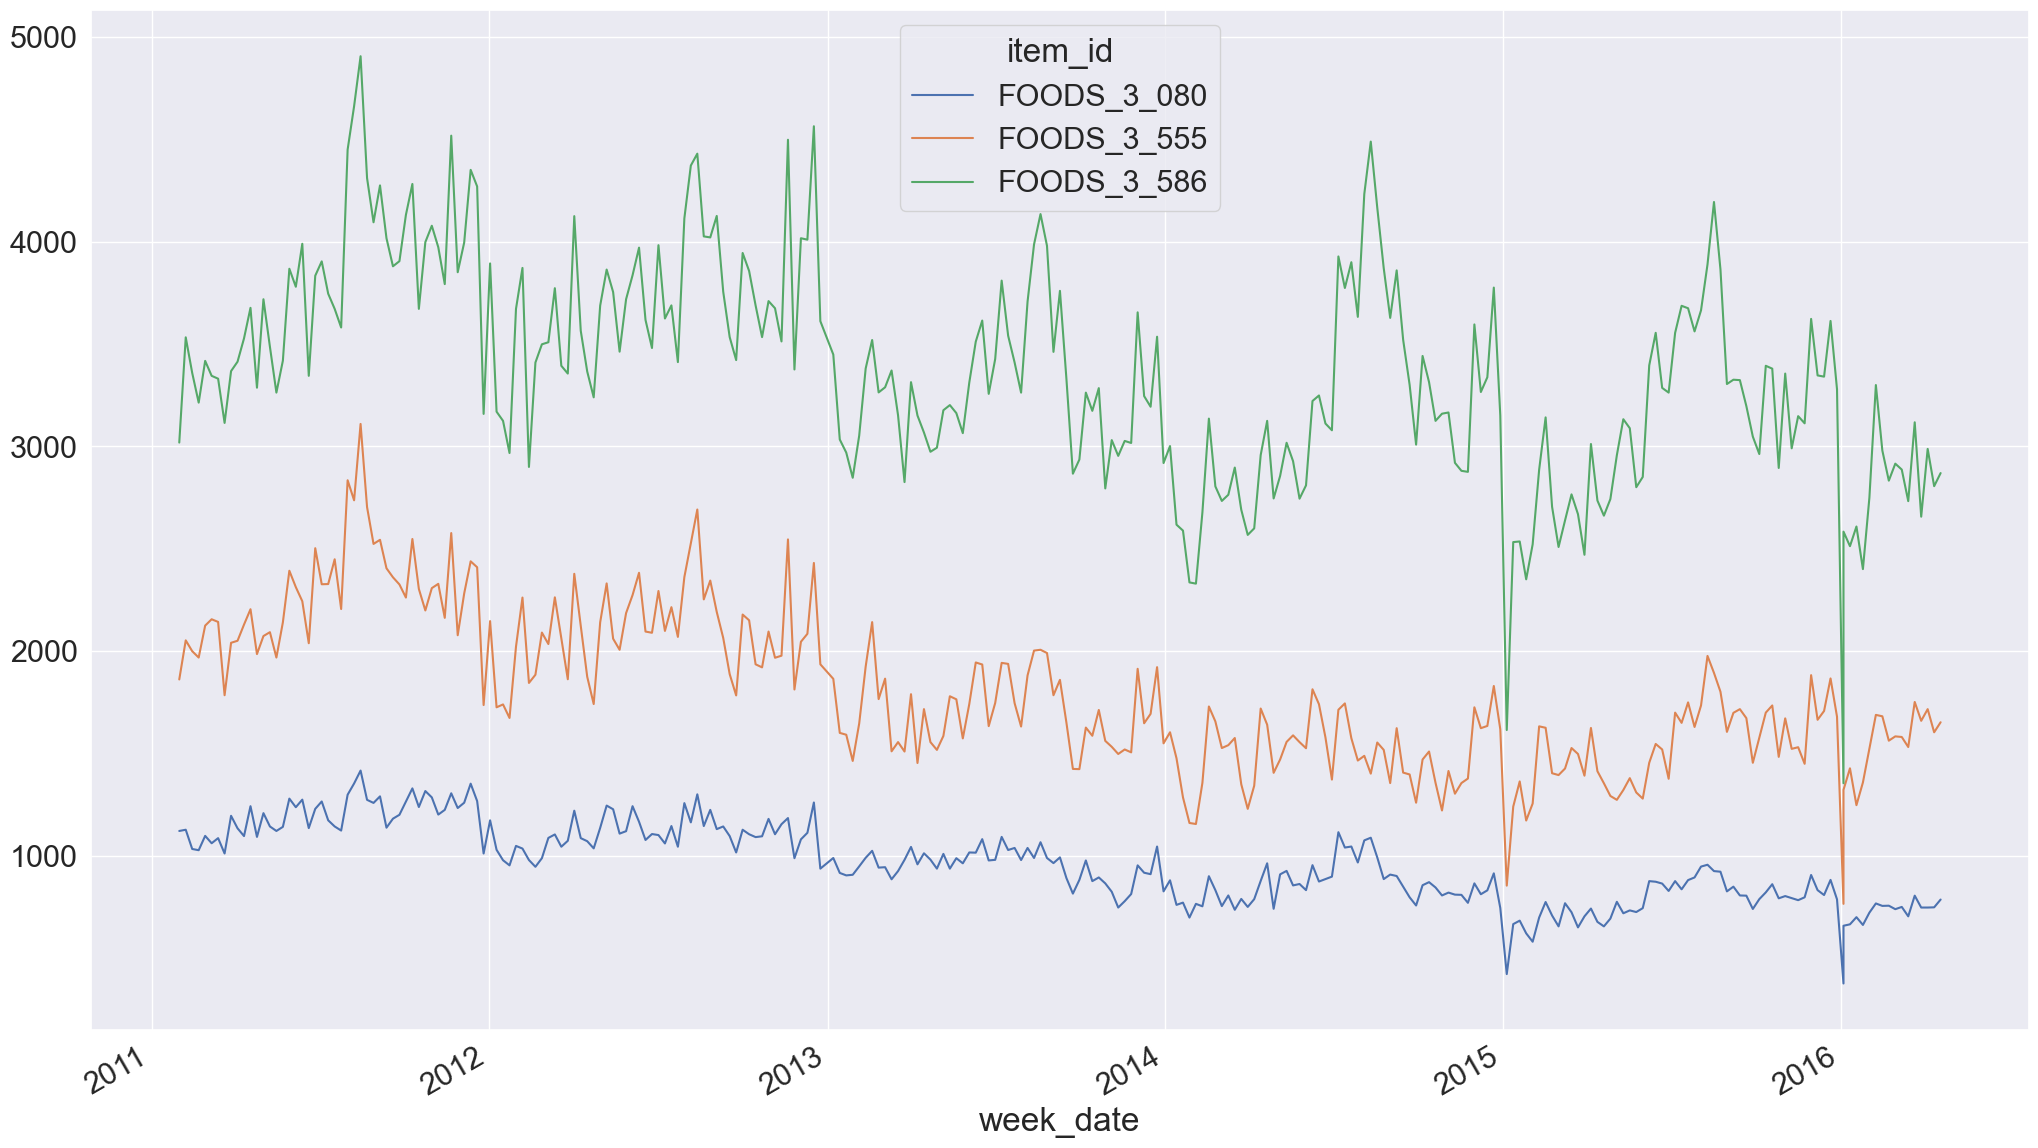
\includegraphics[width=0.8\linewidth]{chapters/05_feature_importance_hierarchy/img/product_sales }
    \centering
    \caption{Total weekly sales for the chosen products}
    \label{fig:product_sales}
\end{figure}


\begin{figure}
    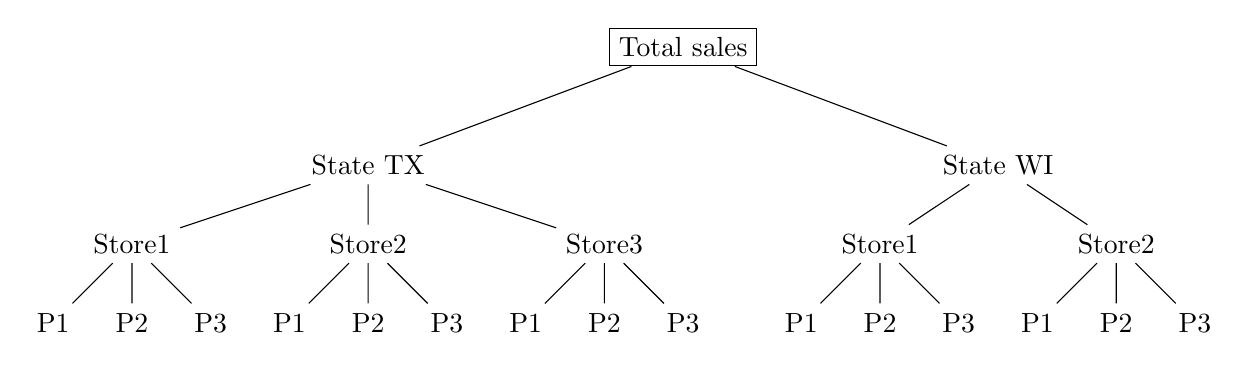
\begin{tikzpicture}
    [level 1/.style={sibling distance=80mm, level distance=15mm},
        level 2/.style={sibling distance=30mm, level distance=10mm},
        level 3/.style={sibling distance=10mm, level distance=10mm}]
        \node[rectangle,draw] {Total sales}
        child {node {State TX}
        child {node {Store1}
        child {node {P1}}
        child {node {P2}}
        child {node {P3}}
        }
        child {node {Store2}
        child {node {P1}}
        child {node {P2}}
        child {node {P3}}
        }
        child {node {Store3}
        child {node {P1}}
        child {node {P2}}
        child {node {P3}}
        }
        }
        child {node {State WI}
        child {node {Store1}
        child {node {P1}}
        child {node {P2}}
        child {node {P3}}
        }
        child {node {Store2}
        child {node {P1}}
        child {node {P2}}
        child {node {P3}}
        }
        };
    \end{tikzpicture}
    \caption{Hierarchical structure of product sales data (P1-3 = Product1-3)} \label{fig:hierarchical_structure}
\end{figure}




\subsection{Model implementation}\label{subsec:model-implementation}
The modelling approach is to build a single global on all series and exogenous variables for bottom-up aggregation.
For creating forecast models, the skforecast\cite{skforecast} library was used.
The base model for hierarchical forecasting was LightGBM~\cite{guolin_ke_highly_2017}
due to its efficiency and also because of its widespread usage in the M5 competition in this data set\cite{makridakis_m5_2022}.
Other ensemble models such as Random Forest or Gradient Boosting Machines could be used as well.
Other reasons for choosing LightGBM are that it can handle categorical variables without the need for one-hot encoding, and that it supports model-specific split and gain-based global feature importance methods.

Hyperparameter tuning was performed using the Optuna library\cite{optuna_2019}, by Bayesian optimisation.
The search space\ref{tab:hyperparam_search_space} was defined for the parameters of the LightGBM model, including the number of predictors, the minimum number of samples in the leaf, and the maximum depth of the tree.
In addition, the number of lagged sales records used as features was included in the search space.
For the search, the data was split into training and validation sets, the last year being the validation set used for backtesting.
The performance of the model was evaluated as a mean square error (MSE) in the validation set for each configuration.
The best configuration found was with 239 estimators and a maximum depth of 26 with a backtesting MSE 4263.01
The lagged sales records used as features were 1, 4, 5, 13, and 52 weeks.
\begin{table}
    \centering
    \begin{tabular}{|l|l|l|}
        \hline
        Parameter          & Search space & Description                                             \\
        \hline
        n\_estimators      & 50-1000      & Number of boosting iterations                           \\
        max\_depth         & 5-50         & Maximum depth of the tree                               \\
        min\_samples\_leaf & 1-10         & Minimum number of samples required to be at a leaf node \\
        num\_lagged\_sales & 4-52         & Number of lagged sales records used as features         \\
        \hline
    \end{tabular}
    \caption{Model hyperparameters search space}
    \label{tab:hyperparam_search_space}
\end{table}

The feature input for the final model is a table with the following columns:
\begin{itemize}
    \item week\_of\_year represented as numerical values (1-52)
    \item sell\_price for the week for the product in the store
    \item num\_of\_events for the week
    \item snap\_days for the week in the state
    \item lag\_\emph{n} for n in [1, 4, 5, 13, 52] representing the sales from the previous weeks
    \item series\_id noted as (\_level\_skforecast) encoded as a numerical value representing the series hierarchy
\end{itemize}





\section{Conclusions}
\label{sec:hierarchical_feature_importance_conclusions}

%TODO:

Main findings





\chapter{Collaborative development for decision support}
\label{ch:collaborative_development}

%\chapter{Collaborative Development for Decision Support}



\section{Best Practices for ML System Development}
\label{sec:best_practices_ml_system_development}
%https://www.researchgate.net/publication/372332486_Towards_Good_Practices_for_Collaborative_Development_of_ML-Based_Systems




\section{Automated delivery of models as services}
\label{sec:automated_delivery_models_services}
%https://www.cs.ubbcluj.ro/~studia-i/journal/journal/article/view/93/93


%

\section{Collaborative Development for Decision Support}
\label{sec:collaborative_development}
https://www.researchgate.net/publication/372332486_Towards_Good_Practices_for_Collaborative_Development_of_ML-Based_Systems





\section{Automated delivery of models as services}
%https://www.cs.ubbcluj.ro/~studia-i/journal/journal/article/view/93/93

Best Practices for Collaborative Development of ML Systems
\begin{itemize}
\item Insights from the development of a demand forecasting system.
\item Discussion on deploying scalable and interpretable ML models in industrial environments.
\end{itemize}




Best Practices for Collaborative Development of ML Systems
\begin{itemize}
    \item Insights from the development of a demand forecasting system.
    \item Discussion on deploying scalable and interpretable ML models in industrial environments.
\end{itemize}


%\section{Challenges in Deploying Explainable AI in Industry}
%\section{Conclusions}


\section{Conclusions}




\chapter{Conclusions and Future Work}
\label{ch:conclusions}

\section{Summary of Contributions}
\label{sec:summary_of_contributions}


\section{Future Research Directions}
\label{sec:future_research_directions}


    \appendix

    \setstretch{1}
    \bibliographystyle{apalike}
%    \bibliography{refs}
    \bibliography{biblography/explain,biblography/hierarhical_importance,biblography/ml,biblography/xai} 
    \label{bib}
    %\bibliography{file1,file2}


\end{document}

